% This is a template for doing homework assignments in LaTeX, cribbed from M. Frenkel (NYU) and A. Hanhart (UW-Madison)

\documentclass{article} % This command is used to set the type of document you are working on such as an article, book, or presenation

\usepackage[margin=1in]{geometry} % This package allows the editing of the page layout. I've set the margins to be 1 inch. 

\usepackage{amsmath, amsfonts}  % The first package allows the use of a large range of mathematical formula, commands, and symbols.  The second gives some useful mathematical fonts.

\usepackage{graphicx}  % This package allows the importing of images
\usepackage{float} % more forced image positions

\usepackage{datetime}

%This allows us to use the theorem and proof environment 
\usepackage{amsthm}
\theoremstyle{plain}
\newtheorem*{theorem*}{Theorem}
\newtheorem{theorem}{Theorem}
\theoremstyle{definition}
\newtheorem*{definition*}{Definition}

%Custom commands.  
\newcommand{\abs}[1]{\left\lvert #1 \right\rvert} %absolute value command

%Custom symbols
\newcommand{\Rb}{\mathbb{R}}




\begin{document}

\begin{center}
    \Large{
        \textbf{Assignment \#3}

        UW-Madison MATH 421
    }
    
    \vspace{5pt}
        
    \normalsize{
        GEOFF YOERGER

        \usdate
        \formatdate{16}{2}{2021}
    }
    
    \vspace{15pt}
\end{center}


\noindent\fbox{\textbf{Exercise \#1:}} Sketch the set of all points $(x,y)$ in the plane satisfying 


\begin{figure}[H]
    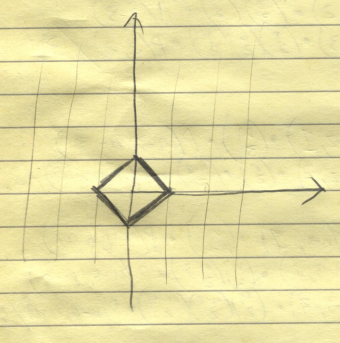
\includegraphics[width=200px]{diamond.png}
    \caption{$\abs{x}+\abs{y}=1$: A diamond}
\end{figure}
\begin{figure}[H]
    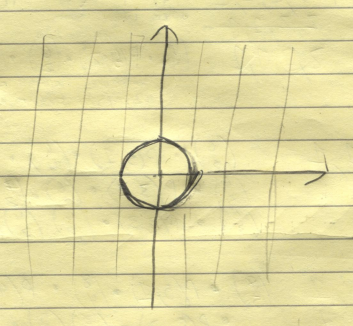
\includegraphics[width=200px]{circle.png}
    \caption{$x^2 + y^2 =1$: A circle}
\end{figure}
\begin{figure}[H]
    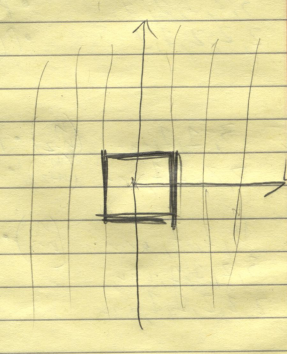
\includegraphics[width=200px]{square.png}
    \caption{$\max\{ \abs{x}, \abs{y} \} = 1$: A square}
\end{figure}

\vspace*{12pt}  %This adds some vertical space. 

\noindent\fbox{\textbf{Exercise \#2:}} Following the instructions on the previous problem: Spivak, Chapter 4, Problem 17 (i) and (ii). 

\begin{figure}[H]
    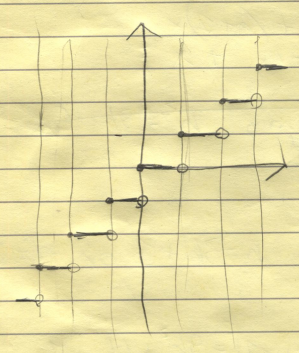
\includegraphics[width=200px]{steps.png}
    \caption{$f(x) = \left \lfloor {x} \right \rfloor$: (i) Steps}
\end{figure}
\begin{figure}[H]
    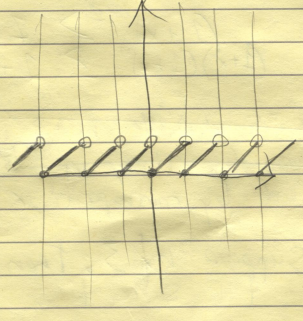
\includegraphics[width=200px]{sawteeth.png}
    \caption{$f(x) = x - \left \lfloor {x} \right \rfloor$: (ii) Sawteeth}
\end{figure}

\vspace*{12pt}  %This adds some vertical space. 


\noindent\fbox{\textbf{Exercise \#3:}} Prove, using only the definition, that $\lim_{x \rightarrow 3} 5x = 15$. 

\begin{proof} 
    Fix $\epsilon > 0$.  Let $\delta = \frac{\epsilon}{5}$. If $0 < |x-3| < \delta$, then

    \begin{align*}
        |f(x) - 15| &= |5x - 15| \\
                    &= 5|x-3| \\
                    &< 5 \delta \\
                    &= 5 \frac{\epsilon}{5} \\
                    &= \epsilon \\
    \end{align*}

    Since $\epsilon$ was arbitrary, $\lim_{x \rightarrow 3} 5x = 15$
\end{proof} 

\noindent\fbox{\textbf{Exercise \#4:}} Prove, using only the definition, that $\lim_{x \rightarrow 2} x^2+2x = 8$. 

\begin{proof} 
    Fix $\epsilon > 0$.  Let $\delta = min\left\{1, \frac{\epsilon}{7} \right\}$. If $0 < |x-2| < \delta$, then

    \begin{align*}
        |f(x) - 8| &= |x^2 + 2x - 8| & & \\
                   &= |x+4| |x-2| & & \\
                   &= |(x-2)+6| |x-2| & & \\
                   &\leq (|x-2| + 6) |x-2| & & \\
                   &< (1 + 6) |x-2| & & \text{Since $|x-2| < 1$} \\
                   &< 7 \frac{\epsilon}{7} & & \text{Since $|x-2| < \frac{\epsilon}{5}$} \\
                   &= \epsilon & & \\
    \end{align*}

    Since $\epsilon$ was arbitrary, $\lim_{x \rightarrow 2} x^2 + 2x = 8$
\end{proof} 

\noindent\fbox{\textbf{Exercise \#5:}} Prove the following theorem: 

\begin{theorem*} If $x$ and $y$ are numbers, then $\abs{\abs{x}-\abs{y}} \leq \abs{x-y}$. 
\end{theorem*}

\begin{proof}
    Notice that $\forall x \forall y:  |x| - |y| \leq |x - y|$.  This was proved in HW2 \S 8.3.  Swapping variables,

    \begin{align*}
        |y| - |x| \leq |y - x| & \Leftrightarrow |y| - |x| \leq |x - y| \\
        & \Leftrightarrow -(|x| - |y|) \\
        & \Leftrightarrow -(|x| - |y|) \leq |x - y| \land |x| - |y| \leq |x-y| \\
        & \Leftrightarrow ||x| - |y|| \leq |x - y| \\
    \end{align*}

\end{proof} 


\noindent\fbox{\textbf{Exercise \#6:}} Spivak, Chapter 5,  16 (a)

\begin{theorem*} If $\lim_{x \to a} f(x) = L$, then $\lim_{x \to a} |f|(x) = |L|$.
\end{theorem*}

\begin{proof} 
    Fix $\epsilon > 0$.  By definition, $\exists \delta$ such that $0 < |x-a| < \delta \implies |f(x) - L| < \epsilon$.
    Suppose $0 < |x-a| < \delta$
    So,
    \begin{align*}
        | |f|(x) - |L| | &= | |f(x)| - |L| | \\
                         &\leq |f(x) - L| \\
                         & < \epsilon \\
    \end{align*}

    Thus, $0 < |x-a| < \delta \implies |f(x) - L| < \epsilon \implies | |f|(x) - |L| | < \epsilon$.

    Since $\epsilon$ was arbitrary, $\lim_{x \to a} |f|(x) = |L|$
\end{proof} 

\noindent\fbox{\textbf{Exercise \#7:}} Spivak, Chapter 5, Problem 12 (a) 

\begin{theorem*} If $\forall x (f(x) \leq g(x))$, $\lim_{x \to a} f(x) = L$ exists, and $\lim_{x \to a} g(x) = M$ exists, then $\lim_{x \to a} f(x) \leq \\lim_{x \to a} g(x)$, equivicantly $L \leq M$
\end{theorem*}

\begin{proof}
    Suppose for a contradiction that $L > M$. By definition, $\lim_{x \to a} (g(x) - f(x)) = M - L$.  Let $\epsilon = L - M$.

    By definition, $\exists \delta > 0$ such that $0 < |x - a| < \delta \implies |g(x) - f(x) + L - M| < \epsilon = L-M$. Thus,

    \begin{align*}
        g(x) - f(x) + L - M & < L - M \\
        g(x) - f(x) & < 0 \\
        g(x) & < f(x) \\
        f(x) & > g(x) \\
    \end{align*}

    But, $f(x) \leq g(x)$, thus a contradiction arises, and $\lim_{x \to a} f(x) \leq \lim_{x \to a} g(x)$
\end{proof} 


\noindent\fbox{\textbf{Exercise \#8:}} Spivak, Chapter 5, Problem 37 (a) 

Define $\lim_{x \to a} f(x) = \infty$ as $\forall N, \exists \delta > 0 \text{ such that } 0 < |x-a| < \delta \implies f(x) > N$.

\begin{theorem*}
    $\lim_{x \to 3} \frac{1}{(x-3)^2} = \infty$
\end{theorem*}

\begin{proof} 
    Fix $N$.  Let $\delta = \frac{1}{\sqrt{N}}$.  If $0 < |x-3| < \delta = \frac{1}{\sqrt{N}}$, then
    \begin{align*}
        |x - 3| = \sqrt{(x-3)^2} & < \frac{1}{\sqrt{N}} \\
        \frac{1}{\sqrt{(x-3)^2}} & > \sqrt{N} \\
        \frac{1}{(x-3)^2} & > N \\
    \end{align*}

    Since $N$ was arbitrary, $0 < |x-3| < \delta \implies \frac{1}{(x-3)^2} > N$, so $lim_{x->a} \frac{1}{(x-3)^2} = \infty$
\end{proof} 





    





    
    
\end{document}
